\documentclass[10pt,a4paper,openany]{article}
\usepackage[latin1]{inputenc}
\usepackage{amsmath}
\usepackage{amsfonts}
\usepackage{amssymb}
\usepackage{graphicx}
\usepackage{listings}
\usepackage{color}
\usepackage[left=2cm,right=2cm,top=3cm,bottom=2cm]{geometry}
\usepackage[numbers,sort&compress]{natbib}
\usepackage[english]{babel}

\setlength{\parindent}{12pt}

\definecolor{mygreen}{rgb}{0,0.6,0}
\definecolor{mygray}{rgb}{0.5,0.5,0.5}
\definecolor{mymauve}{rgb}{0.58,0,0.82}

\lstset{ 
	backgroundcolor=\color{white},   % choose the background color; you must add \usepackage{color} or \usepackage{xcolor}; should come as last argument
	basicstyle=\footnotesize,        % the size of the fonts that are used for the code
	breakatwhitespace=false,         % sets if automatic breaks should only happen at whitespace
	breaklines=true,                 % sets automatic line breaking
	captionpos=b,                    % sets the caption-position to bottom
	commentstyle=\color{mygreen},    % comment style
	deletekeywords={...},            % if you want to delete keywords from the given language
	escapeinside={\%*}{*)},          % if you want to add LaTeX within your code
	extendedchars=true,              % lets you use non-ASCII characters; for 8-bits encodings only, does not work with UTF-8
	firstnumber=01,                	 % start line enumeration with line 1000
	frame=single,	                 % adds a frame around the code
	keepspaces=true,                 % keeps spaces in text, useful for keeping indentation of code (possibly needs columns=flexible)
	keywordstyle=\color{blue},       % keyword style
	language=Python,                 % the language of the code
	morekeywords={*,...},            % if you want to add more keywords to the set
	numbers=left,                    % where to put the line-numbers; possible values are (none, left, right)
	numbersep=5pt,                   % how far the line-numbers are from the code
	numberstyle=\tiny\color{mygray}, % the style that is used for the line-numbers
	rulecolor=\color{black},         % if not set, the frame-color may be changed on line-breaks within not-black text (e.g. comments (green here))
	showspaces=false,                % show spaces everywhere adding particular underscores; it overrides 'showstringspaces'
	showstringspaces=false,          % underline spaces within strings only
	showtabs=false,                  % show tabs within strings adding particular underscores
	stepnumber=1,                    % the step between two line-numbers. If it's 1, each line will be numbered
	stringstyle=\color{mymauve},     % string literal style
	tabsize=2,	                     % sets default tabsize to 2 spaces
	title=\lstname                   % show the filename of files included with \lstinputlisting; also try caption instead of title
}

\author{Oscar Alejandro Hern�ndez L�pez}
\title{Homework Assignment 1: Network Flows}
\date{}

\begin{document}
	
	\maketitle
	
	\section*{Undirected acyclic graph}
	Consider the general index of a book. Such index is a tree and has a relation with the chapters and these with the sections. The root, the node \textit{Book}, has three subtrees which are the chapters \textit{C1},\textit{C2} and \textit{C3}. This three nodes are the inheritance of the node named \textit{Book}. Also we have two subtrees with non trivial relations, for example \textit{C2} has another three subtrees which represent sections \textit{s2.1}, \textit{s2.2}, \textit{s2.3.} \citep{datos1}
	
	\lstinputlisting[language=Python]{01undirected_acyclic_graph.py}
	
		\begin{center}
			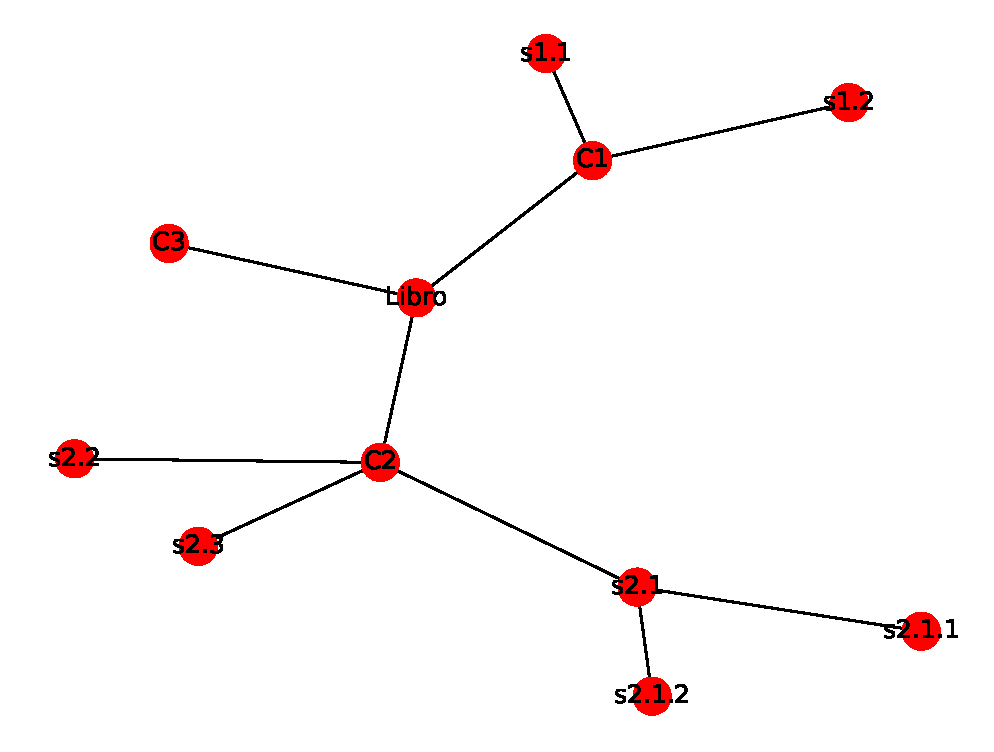
\includegraphics[scale=0.8]{Graph01}
		\end{center}
		
	\section*{Undirected cyclic graph}
	In this situation we have five cities. Cities \textit{A} and \textit{B} are separated by a distance of 50 km, between cities \textit{B} and \textit{C} are 20 km and there is 30 km and 35 km between cities \textit{C} and \textit{D}, and \textit{D} and \textit{E}, respectively. The nearest distance is between cities \textit{A} and \textit{E}, with 15 km. \citep{grafo2}
	
		\lstinputlisting[language=Python]{02undirected_cyclic_graph.py}
	
		\begin{center}
			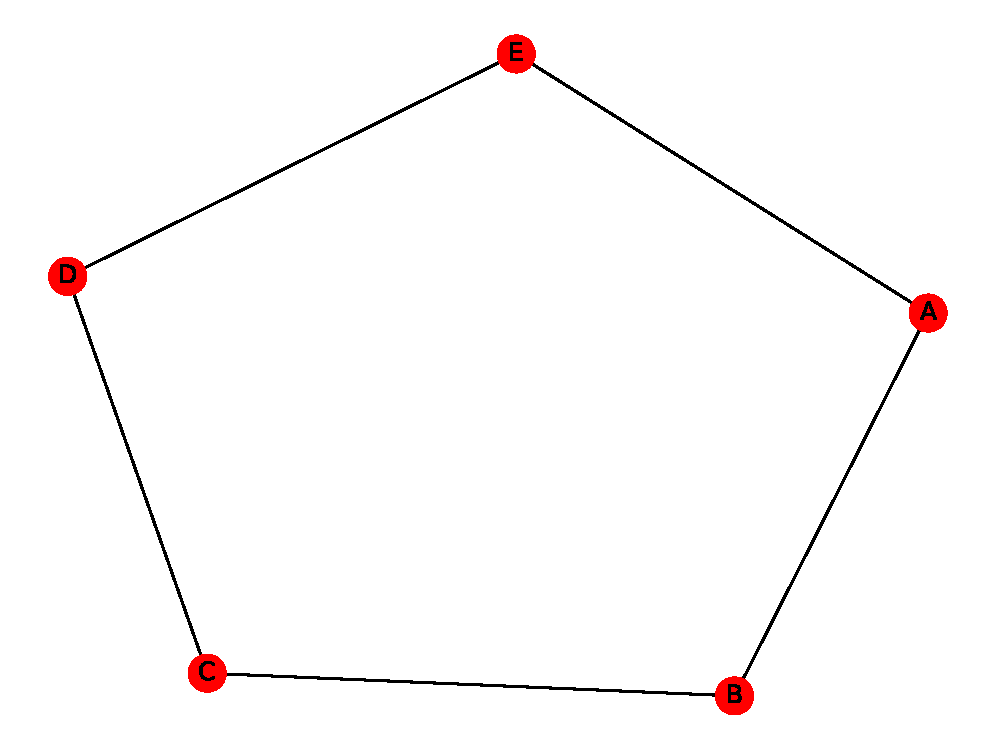
\includegraphics[scale=0.8]{Graph02}
		\end{center}

	\newpage
	
	\section*{Undirected reflexive graph}
	The example shows relationships between republics, we can call it cluster (\textit{0},\textit{1} and \textit{2}). Clusters \textit{3} and \textit{4} are other republics that have significant ties with \textit{0}, but almost no ties with anyone else. In case of republic \textit{3} in addition to other relationships, can do other local relations or trades.  \citep{reflexivo1}
	
		\lstinputlisting[language=Python]{03undirected_reflexive_graph.py}
		
		\begin{center}
			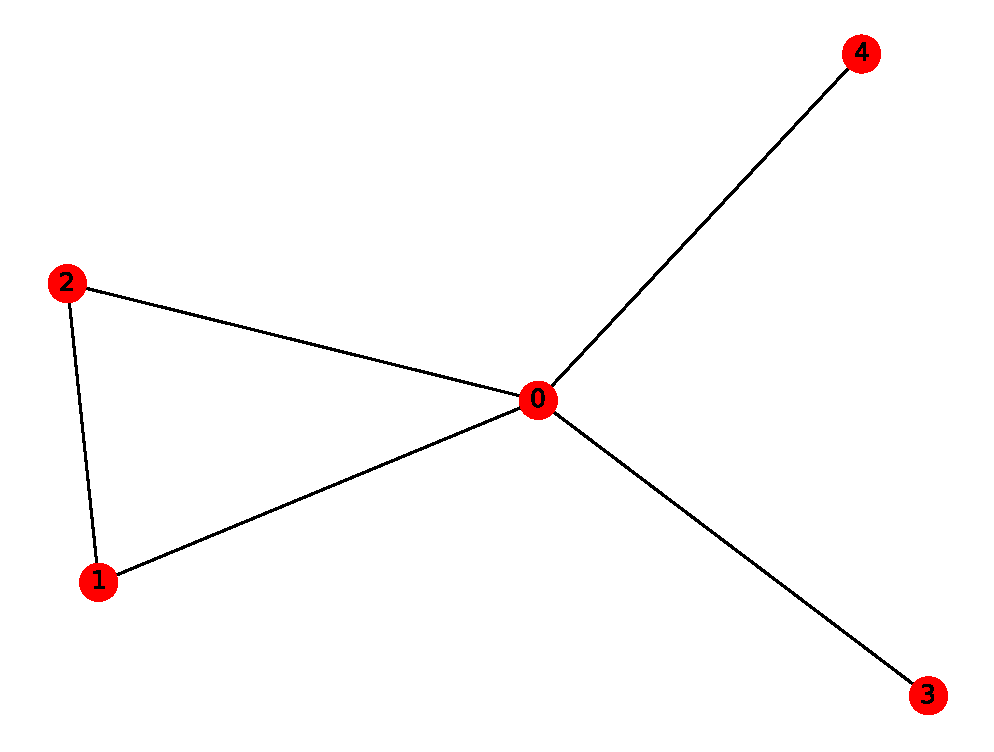
\includegraphics[scale=0.8]{Graph03}
		\end{center}
	
	\newpage
	
	\section*{Directed acyclic graph}
	The example is about the Bayes's basic structure, which begins by a tree structure with its predictive variables and later connect the \textit{X} variable with every single predictive variables $R_{n}$. In this acyclic directed graph every node represents a variable and every edge a probabilistic dependence, specifying the conditional probability of this variables with its sources. Every connections are identified by simple path that does not repeat vertices. \citep{graph2}
		
		\lstinputlisting[language=Python]{04directed_acyclic_graph.py}
	
		\begin{center}
			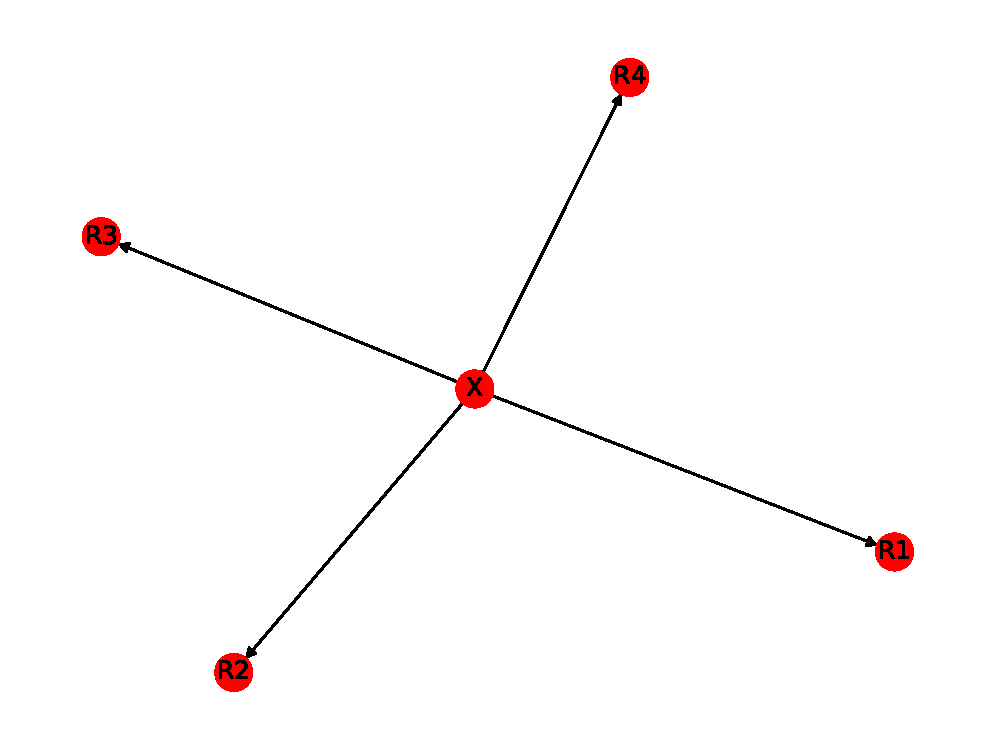
\includegraphics[scale=0.8]{Graph04}
		\end{center}
	
	\newpage
	
	\section*{Directed cyclic graph}
	This situation consists in a fleet of homogeneous vehicles which need to distribute the jobs to respective customers. The routing graph is the set of nodes where a node \textit{DEPOT} represents the main facility where the vehicles are loaded. The rest of nodes denote the rest of the customers. Each job corresponds to a unique customer. The number of vehicles is limited and each customer order needs to be delivered. Tours are allowed to visit multiple customers. \citep{kesen2019integrated}
	
		\lstinputlisting[language=Python]{05directed_ciclic_graph.py}
	
		\begin{center}
			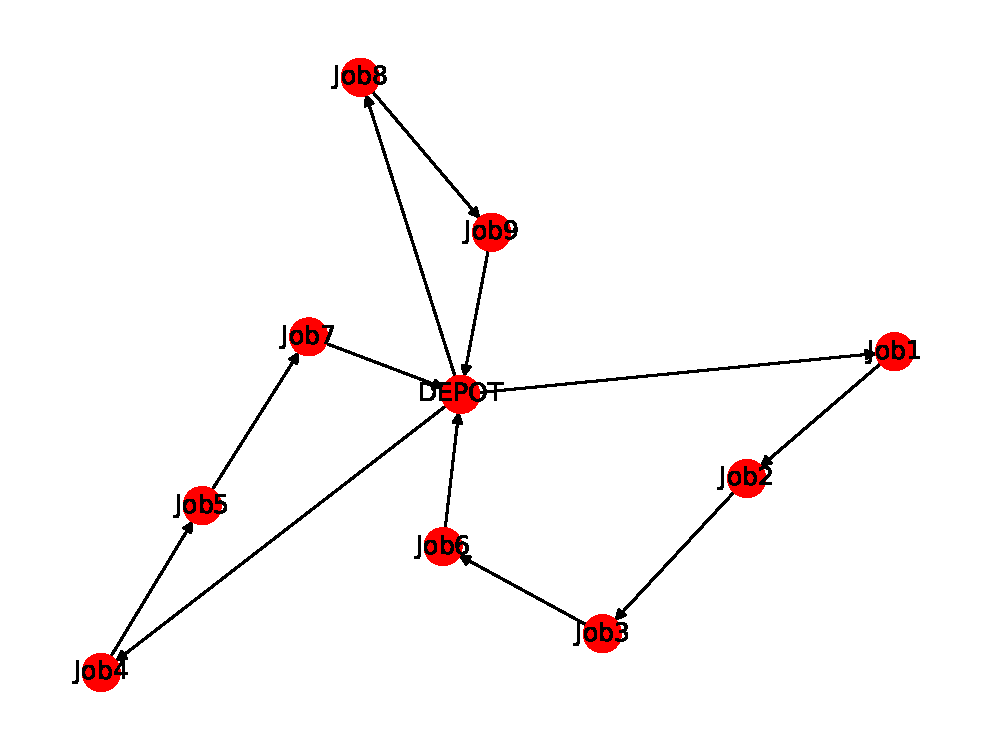
\includegraphics[scale=0.8]{Graph05}
		\end{center}
	
	\newpage
	\section*{Directed reflexive graph}
	A global courier has to deliver some goods in 4 countries. For technical issues and distances between destinations a transport can only visit at most two destinations. Once it visit the costumers has to return to depot in order to begin maintenance for the next departure. In case an order  had started from \textit{DEPOT} and is cancelled the transport can return. \citep{graphdatabase}
	
		\lstinputlisting[language=Python]{06directed_reflexive_graph.py}
	
		\begin{center}
			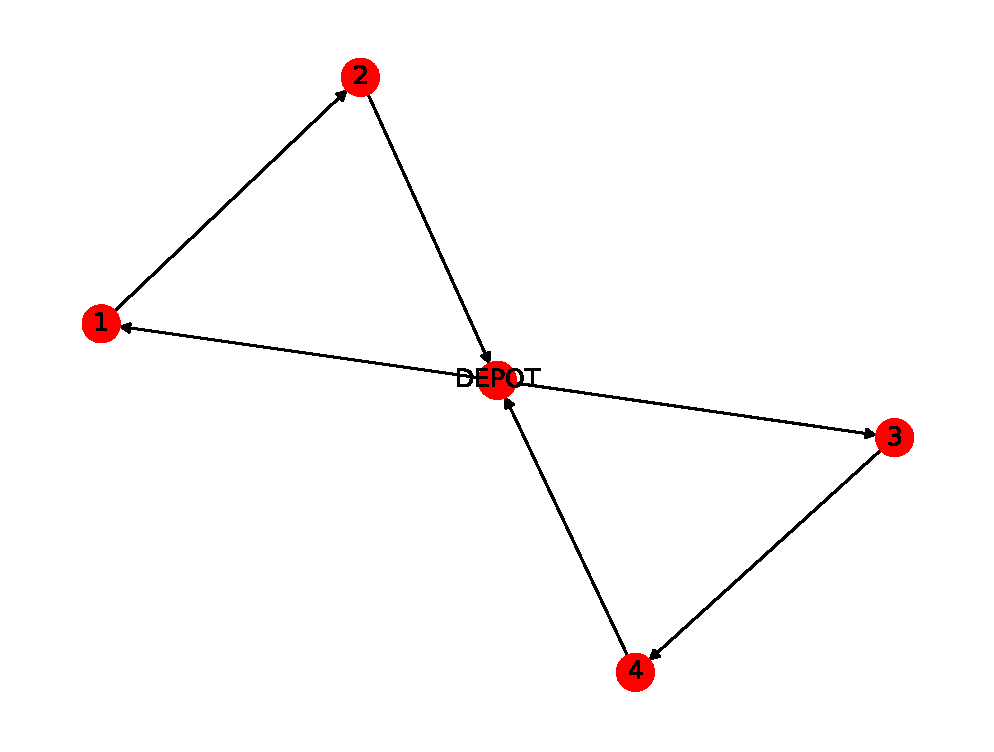
\includegraphics[scale=0.8]{Graph06}
		\end{center}
	
	\newpage		
	
	\section*{Undirected acyclic multigraph}
	Here we have a set of 5 tasks: \textit{X}, \textit{Y}, \textit{Z}, \textit{V}, \textit{W} which need to be done to run a system. We also can consider we have 6 processors we need to assign to each task. Due to complexity of activities \textit{X} and \textit{Y} we shall assign two processors to execute at least one of them. This way we have two different relations between \textit{X} and \textit{Y}, and only one relation between the other tasks. \citep{ferro1996asignacion}
	
		\lstinputlisting[language=Python]{07undirected_acyclic_multigraph.py}
		
		\begin{center}
			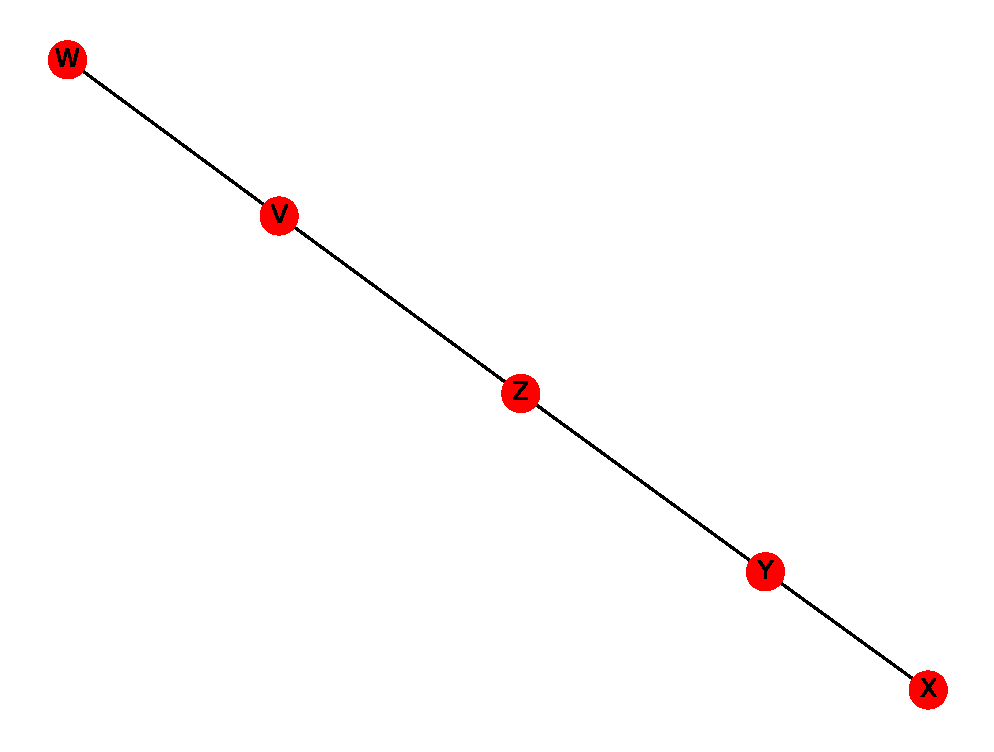
\includegraphics[scale=0.8]{Graph07}
		\end{center}
	
	\section*{Undirected cyclic multigraph}
	This example is about a city divided in five zones. This five zones are united by six roads and people of the city, wants to cross each of the paths only once and end in the same place where they have started.
	\citep{stein1961mathematician}
	
		\lstinputlisting[language=Python]{08undirected_cyclic_multigraph.py}
	
		\begin{center}
			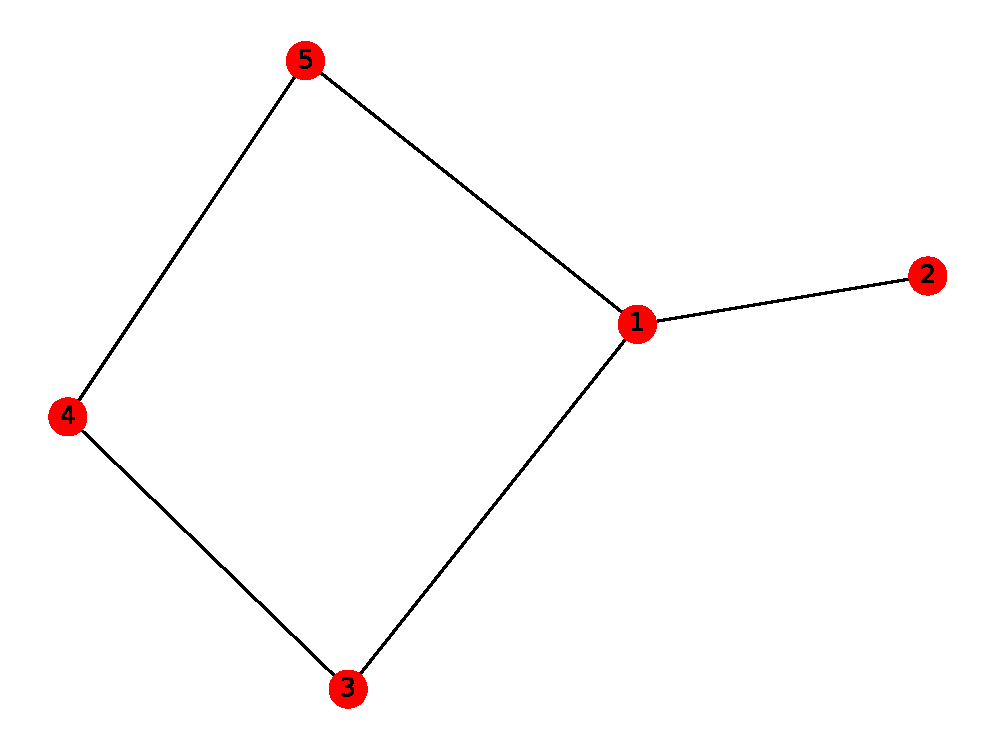
\includegraphics[scale=0.8]{Graph08}
		\end{center}
	
	
	\section*{Undirected reflexive multigraph}
	Assume we have five workstations in a plant. The product needs to go through all the stations not matter the order or a secuence. We know station \textit{A} has a section of quality control where the product is tested, and if it is not good enough needs to be reprocessed. Also relations in sections \textit{A}-\textit{B} or \textit{A}-\textit{C} can be choosing two paths, while relations \textit{B}-\textit{C}, \textit{B}-\textit{D},\textit{C}-\textit{E} and \textit{D}-\textit{E} can only be performed by one path.  \citep{west2001introduction}
	
		\lstinputlisting[language=Python]{09undirected_reflexive_multigraph.py}
		
		\begin{center}
			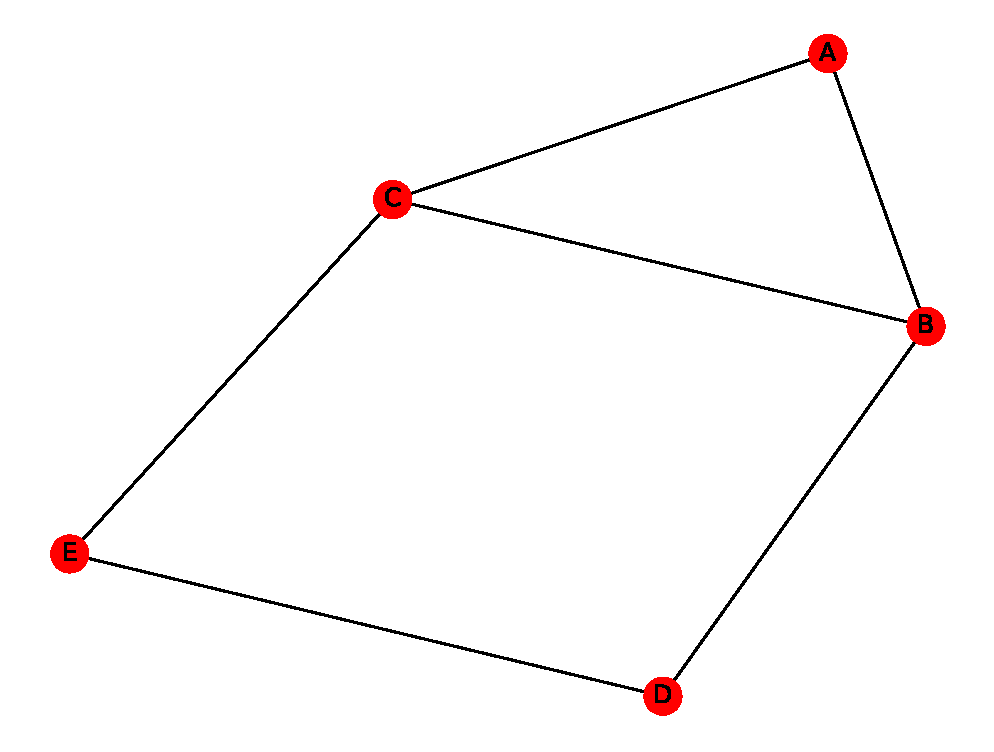
\includegraphics[scale=0.8]{Graph09}
		\end{center}
	
	\section*{Directed acyclic multigraph}
	Certain company has 5 departments which some of them share relations in terms of information flow. Let say $x_{2}$ is the central deparment and needs to have a complete feedback. Deparments  $x_{1}$ and $x_{5}$ has to share information only with the central deparment, the same as $x_{3}$, with the difference of two subjects. Whereas the department $x_{4}$ has to share information to departments $x_{3}$ and the central one.
	\citep{capcha2016teoria}
	
		\lstinputlisting[language=Python]{10directed_acyclic_multigraph.py}
	
		\begin{center}
			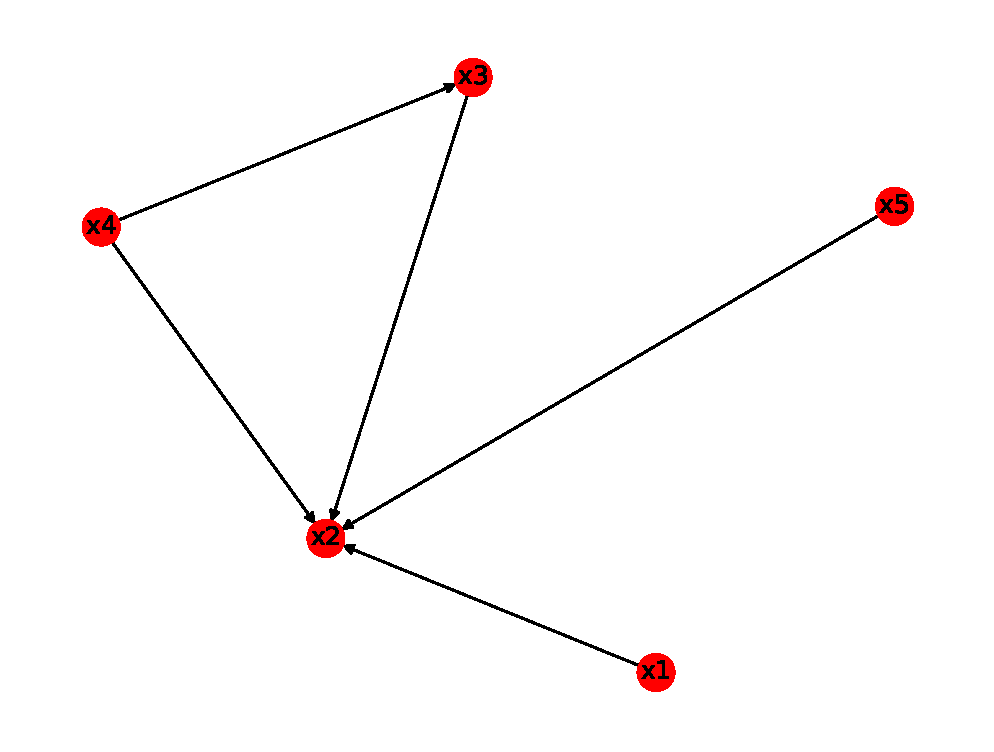
\includegraphics[scale=0.8]{Graph10}
		\end{center}
	
	\section*{Directed cyclic multigraph}
	A student wants to spend his summer vacations in 5 states of Mexico: Coahuila, Sonora, Guanajuato, Veracruz and Quintana Roo. He will start in Coahuila, and  then he will go to Sonora to visit his family. Then he will return to Coahuila to travel with his friends to Guanajuato, Veracruz and Quintana Roo in that order.  He has the chance to return to Coahuila once he finish the visits. \citep{scielo2010}
	
		\lstinputlisting[language=Python]{11directed_cyclic_multigraph.py}
	
		\begin{center}
			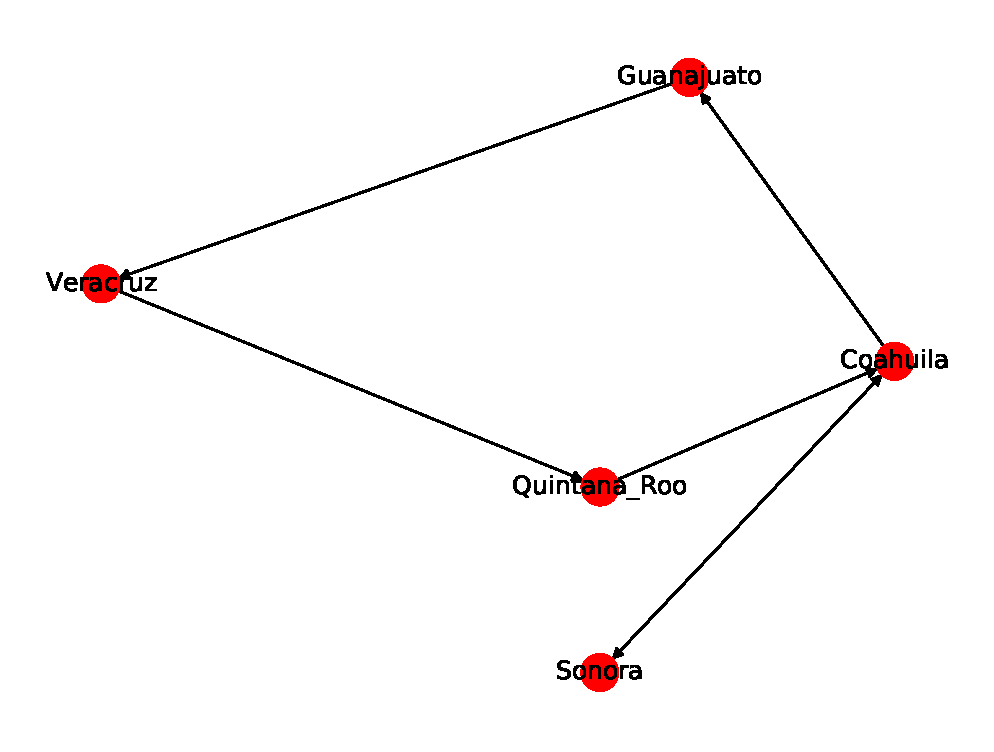
\includegraphics[scale=0.8]{Graph11}
		\end{center}
	
	\section*{Directed reflexive multigraph}
	A logistic company has to deliver 4 orders of pallets from the depot to its warehouses. In order to speed operations up it will allocate 2 trucks to deliver in \textit{warehouse1} and will use only one truck in the other warehouses. In order to keep stock, it will have to produce in-place a small quantity of pallets for inventory security and transport it to the small warehouse at the depot.\citep{multi2005jesus}
	
		\lstinputlisting[language=Python]{12directed_reflexive_multigraph.py}
	
		\begin{center}
			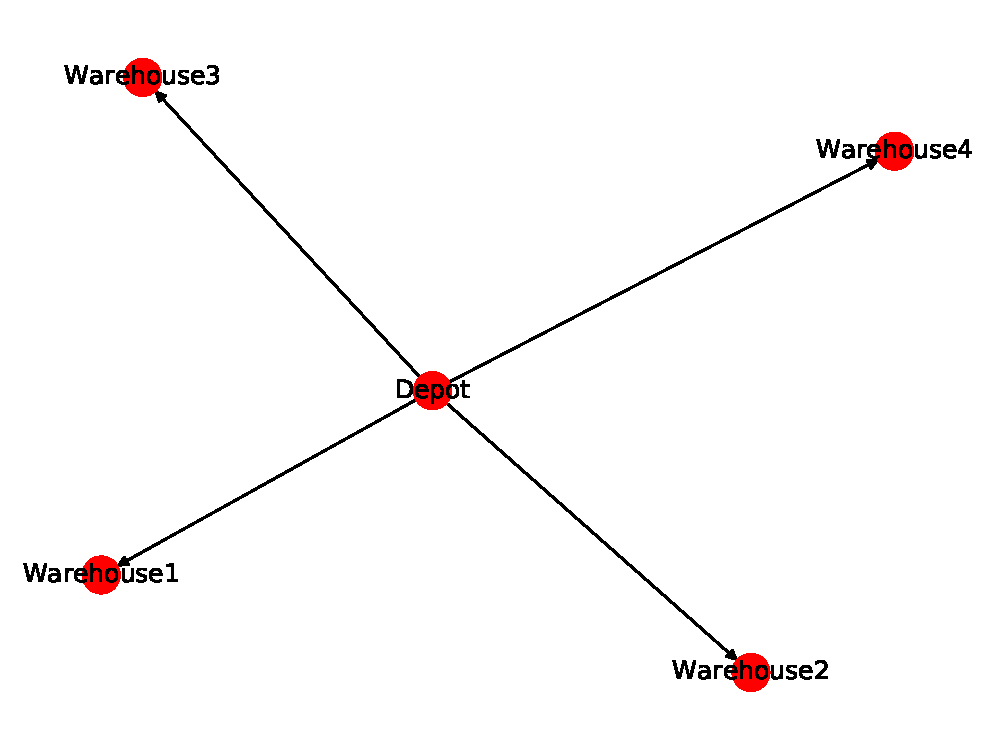
\includegraphics[scale=0.8]{Graph12}
		\end{center}

	\bibliography{document}
	\bibliographystyle{plainnat}
	
\end{document}